\chapter{Informationsbeschaffung}
\label{chap:Informationsbeschaffung}
Dieses Kapitel bietet fundamentale physikalische Gegebenheiten, sowie die relevanten Eigenheiten des verwendeten \ac{PIR}-Sensors. Da es sich um eine bildgebendes Messprinzip handelt, werden des Weiteren geometrische Aspekte erläutert. Schlussendlich bietet dieses Kapitel auch nötige Informationen über das Messobjekt bzw. die Messumgebung geliefert.

\section{Grid-Eye AMG8834}
\label{sec:AMG8834}

Der verwendete Panasonic AMG8834 ist ein bildgebender \ac{MEMS}-Sensor, der mit insgesamt 64 temperaturempfindlichen Thermosäulenelementen ausgestattet ist. Diese sind als 8x8 Pixelmatrix auf den Chip aufgebracht. In Abbildung \ref{fig:Explosionsdarstellung} ist der Aufbau des Sensors dargestellt. Nachfolgende Angaben sind auch dem Datenblatt zu entnehmen, wenn nicht anders angegeben.
 
\begin{figure}[H]
	\centering
	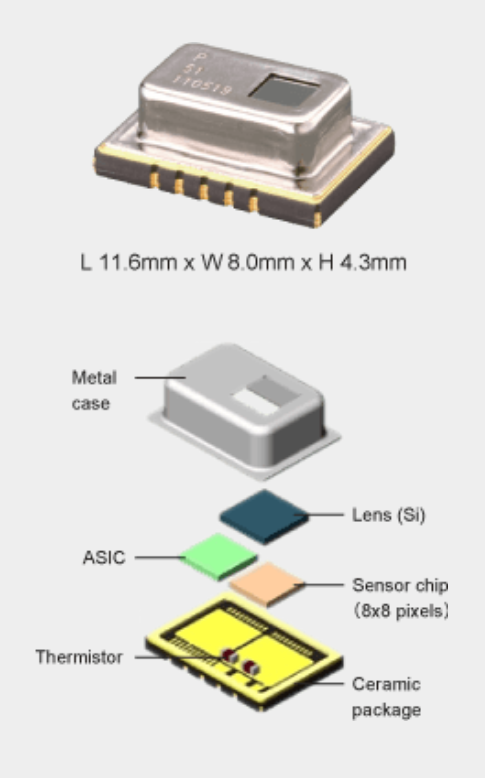
\includegraphics[width=0.3\textwidth]
	{fig/grid_eye_aufbau.PNG}
	\caption[Aufbau des AMG8834 Sensors]{Aufbau des AMG8834 Sensors} \protect\cite{AMG8834}
	\label{fig:Explosionsdarstellung}
\end{figure}
Die eintreffenden Infrarotwellen werden durch die Siliziumlinse, welche einen \ac{FOV} von 60$^\circ$ besitzt, gefiltert. Dabei durchdringen lediglich langwellige Infrarotstrahlungen mit den Wellenlängen 8-13 $\mu$m die Linse. Dies entspricht dem dritten atmosphärischen Fenster.

In Abbildung \ref{fig:SchemaAMG8834} ist das Prinzipschema des Sensors darstellt. Die Umwandlung der Infrarotwellen in die Thermospannung wird im Unterkapitel \ref{subsec:seebeck} detailliert erläutert, daher wird in diesem Abschnitt darauf verzichtet. Die Signale der einzelnen Pixel werden durch die \ac{ASIC} des \ac{MEMS}-Sensor verarbeitet. Die selektierte Thermospannung wird verstärkt, mit dem integrierten Thermistor verglichen und mit dem \ac{ADC} gewandelt. Durch die hohe interne Verstärkung besitzt der Sensor bei normalen Bedingungen\footnote[1]{Umgebungstemperatur 0-80 $^\circ$C bei Luftfeuchtigkeit 15-85\%} eine Genauigkeit von +/- 3°C. 

\begin{figure}[H]
	\centering
	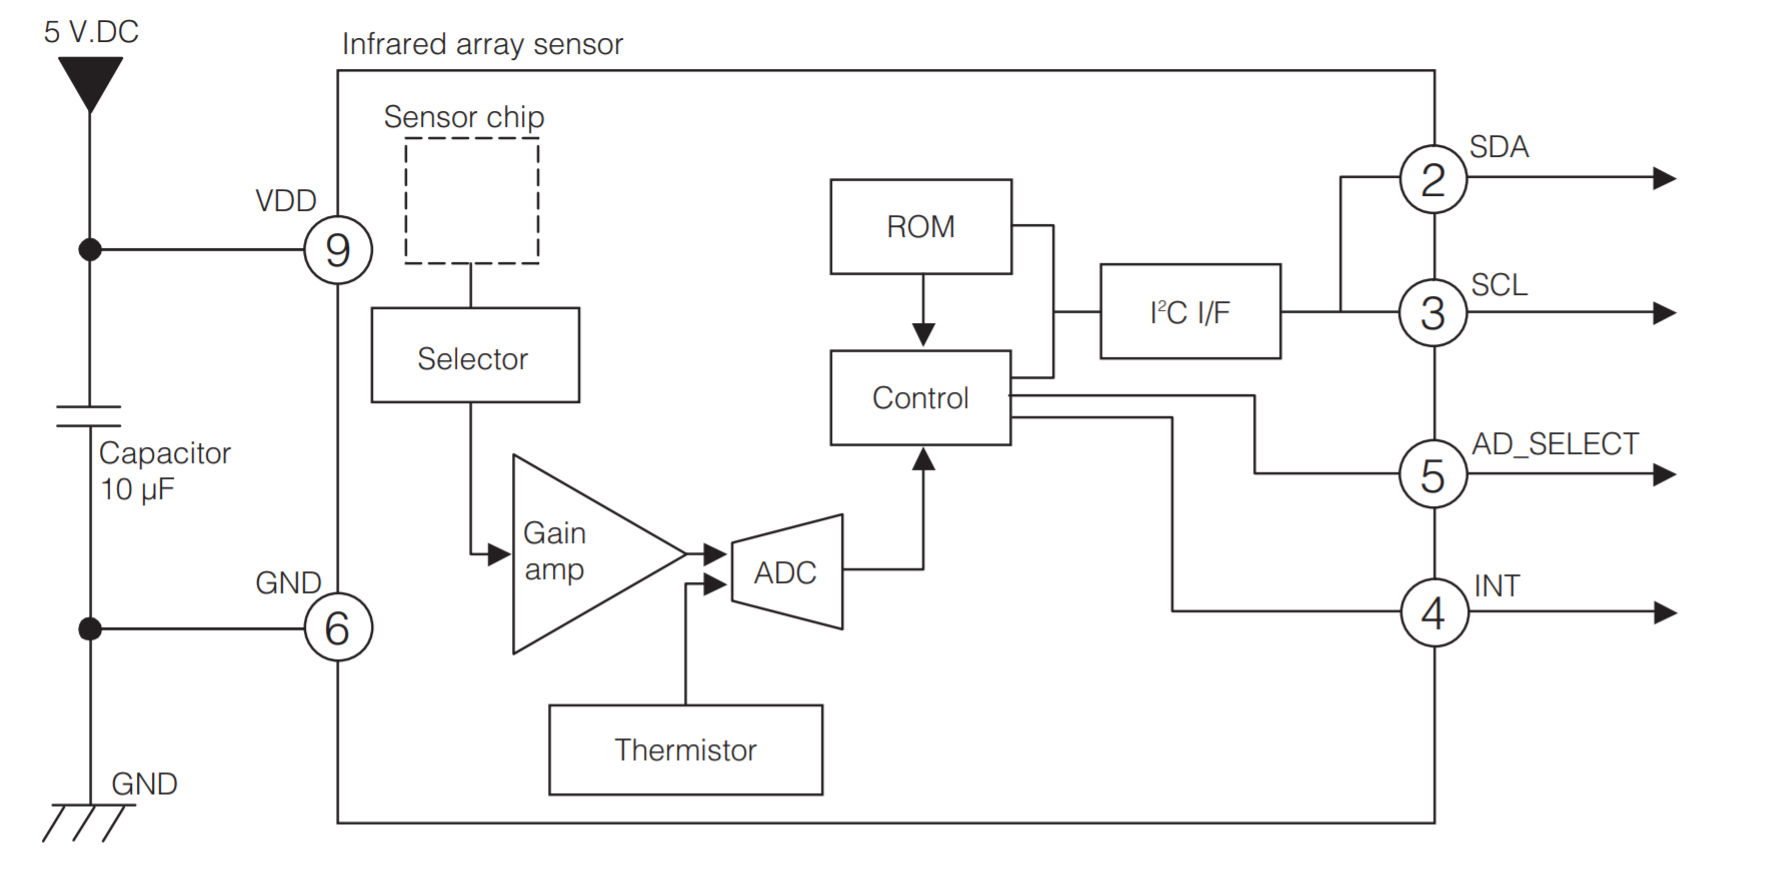
\includegraphics[width=0.75\textwidth]
	{fig/Circuit_AMG8834.PNG}
	\caption[Schema des AMG8834 Sensors]{Schema des AMG8834 Sensors} \protect\cite{AMG8834}
	\label{fig:SchemaAMG8834}
\end{figure}
 
Über die \ac{I2C}-Schnittstelle lassen sich die Werte der Thermoelemente und der Thermistoren je aus 2 Register auslesen. Die Messwerte werden alle 100 ms aktualisiert. Dabei werden lediglich 12 Bit pro Pixel für die Temperaturregister genutzt. Dies führt zu der kleinsten unterscheidbaren Größe von 0.25 $^\circ$C. Die Thermistorregister lassen sich mit der Auflösung von 0.625 $^\circ$C unterscheiden. In Abbildung \ref{fig:SchemaAMG8834} ist klar ersichtlich, dass die Umgebungstemperatur, bzw. die Temperatur, welche vom Thermistor gemessen wird, direkten Einfluss auf die Pixelwerte besitzt. Variieren die Thermistorwerte aufgrund von Raumtemperaturschwankungen entstehen bei den Pixelwerten dadurch entspprehende Schwankungen.

\section{Physikalische Aspekte}
\label{sec:Physik}
Dieser Abschnitt erläutert auf kurze und prägnante Weise, physikalischen Aspekte die dem Sensor zu Grunde liegen. Dies bietet die Grundlage für die Bestimmung der Störquellen und das Verhalten des Sensors bei entsprechenden äußeren Einwirkungen. Die Tabelle \ref{tab:Legende Physikalische Grössen} gibt die Bezeichnungen der nachfolgenden Formeln wieder.

\begin{table}[H]
	\centering
	\begin{tabular}{l|c|c}
		\rowcolor{gray} Grösse &  Bezeichnung  & Einheit \\
		\hline 
		Thermospannung &  $ U_{t}$ & $J$  \\ 
		\rowcolor{gray} Thermokraft P/N -Silizium  & $\alpha_{p},\alpha_{n}$ & $V/K$\\	
		Temperatur P/N -Silizium &  $T_{p},T_{n}$ & $V/K$ \\
		\rowcolor{gray}Wärmestrom &  $\dot{Q}$ & $J$  \\ 
		Emission & $\epsilon$ & $-$\\	
		\rowcolor{gray}Reflektion &  $\rho $ & $-$ \\
		Transmission & $\tau$ & $-$\\
		\rowcolor{gray}Absoprtion &  $\alpha$ & $-$  \\ 
		Strahlungsleistung & $\dot{Q}$ & $W$\\
		\rowcolor{gray}spektrale spezifische Ausstrahlung &  $M_{\lambda }$ & $W/sr$\footnote[2]{Steradiant: Messeinheit für den Raumwinkel} \\
		Planksches Wirkungsquantum &  $ h$ & Js \\ 
		\rowcolor{gray} Lichtgeschwindigkeit im Vakuum & $c $ & $ m/s$ \\ 
 		Stefan-Boltzmann-Konstante & $\sigma$ & $ W/m^2K^2 $ \\ 
	\end{tabular}
	\caption{Legende physikalische Grössen Konzeptzeichnungen}
	\label{tab:Legende Physikalische Grössen} 
\end{table} 


\subsection{Seebeck-Effekt}
\label{subsec:seebeck}
In Abbildung \ref{fig:AufbauThermo} ist ein einzelnes Pixel funktionell dargestellt. Die durch die konvexe Linse gesammelten Infrarotstrahlen verursachen auf den dünnen Thermosäulenflächen (2), dass die Oberfläche erwärmt wird. Es entsteht zwischen der erwärmten, n-dotierten Siliziumschicht (4) und der kühleren p-dotierten Siliziumschicht (6) ein Temperaturgefälle.   

\begin{figure}[H]
	\centering
	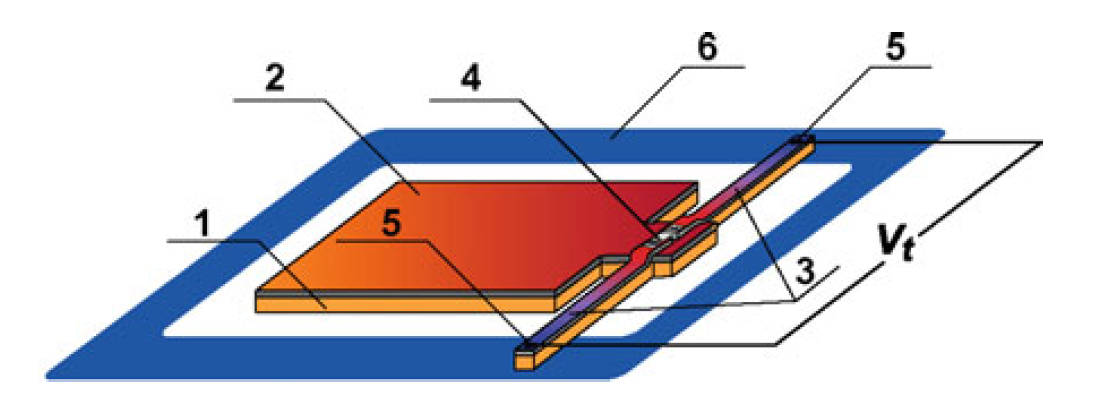
\includegraphics[width=0.6\textwidth]
	{fig/Mems_Thermopile.PNG}
	\caption[Aufbau Thermosäulenelement]{Aufbau Thermosäule} \protect\cite{AMG8834}
	\label{fig:AufbauThermo}
\end{figure}

Durch die unterschiedlichen Thermokräfte (auch Seebeckkoeffizienten) der zwei Halbleitermaterialien entsteht ein Potentialunterschied, den man an den Punkten 3 und 5 abgreifen kann. Diese Spannung $U_{t}$ ist die Grundlage des Messprinzips und wird mit Formel \ref{eq1} \protect\cite{AMG8834} beschrieben.

\begin{equation}
\label{eq1}
U_{t} = (\alpha_{p} + \alpha_{n})*(T_{p}+T_{n})
\end{equation}
\myequations{Seebeck-Effekt}

\subsection{Strahlungstheorie}
\label{subsec:Strahlungstheorie}
Das vorherige Unterkapitel erläutert die Funktion des Sensors als Infrarotempfänger. Nicht unwesentlich ist weiter die Betrachtung des Senders. Grundsätzlich gilt, jeder Körper, der eine Temperatur oberhalb des absoluten Nullpunkt aufweist, strahlt Wärmestrahlung im Infrarotbereich ab. 

Im Allgemein wird für die Betrachtung vom Plank'schen Strahlungsgesetz ausgegangen. Nach dieser gilt für eine spektrale spezifische Ausstrahlung eines Schwarzkörpers mit der Temperatur T folgende Formel \protect\cite{Thermoformeln}:

\begin{equation}
\label{eq2}
M_{\lambda } = \frac{2\pi h c^2 }{\lambda^5}*\frac{1}{e^\frac{hc}{\lambda k_{B} T}-1}
\end{equation}
\myequations{Plank'sches Strahlungsgesetz}

Wie in der Formel ersichtlich ist die Ausstrahlung eines schwarzen Körper mit 5. Potenz von der Wellenlänge und exponentiell von der Temperatur abhängig. Durch die Siliziumlinse des Sensors werden Störquellen, welche andere Wellenlängen aufweisen, gefiltert. Dies ist vor allem bei Lichtquellen ein relevante Eigenschaft. Da dessen Spektrum sich bedeutend tiefer \footnote[3]{Bereich 0.4$\mu$m - 2 $\mu$m} befinden, könen Strahlungseinflusse von herkömmlichen Lichtquellen ignoriert werden kann.

Das Stefan-Boltzmann-Gesetz \protect\cite{Thermoformeln} gibt die Strahlungsintensität $\dot{Q}$ eines idealen Temperaturstrahlers an. Diese Formel bietet für die Anwendung die relevanten Erkenntnisse.


\begin{equation}
\label{eq3}
\dot{Q} = \frac{\mathrm{d} Q}{\mathrm{d} t} = \epsilon *\sigma * A * T_{obj}^4
\end{equation}
\myequations{Wärmestrahlung}

Diese Formel zeigt auf, dass die Wärmestrahlung eines Körpers im wesentlichsten (mit 4. Potenz) von der eigenen Temperatur abhängig ist. Die Fläche A ist lediglich proportional. Dies verursacht, dass bereits flächenmäßig kleine, jedoch stark erwärmte Objekte im Messbereich einen bedeutenden Einfluss auf die Messresultate liefern können. Zusätzlich verursachen Wärmequellen im nahen Umfeld des Sensors Abweichungen auf die Messresultate. In Abbildung \ref{fig:AufbauThermo} ist das Sender/Empfänger-Prinzip dargestellt.

\begin{figure}[H]
	\centering
	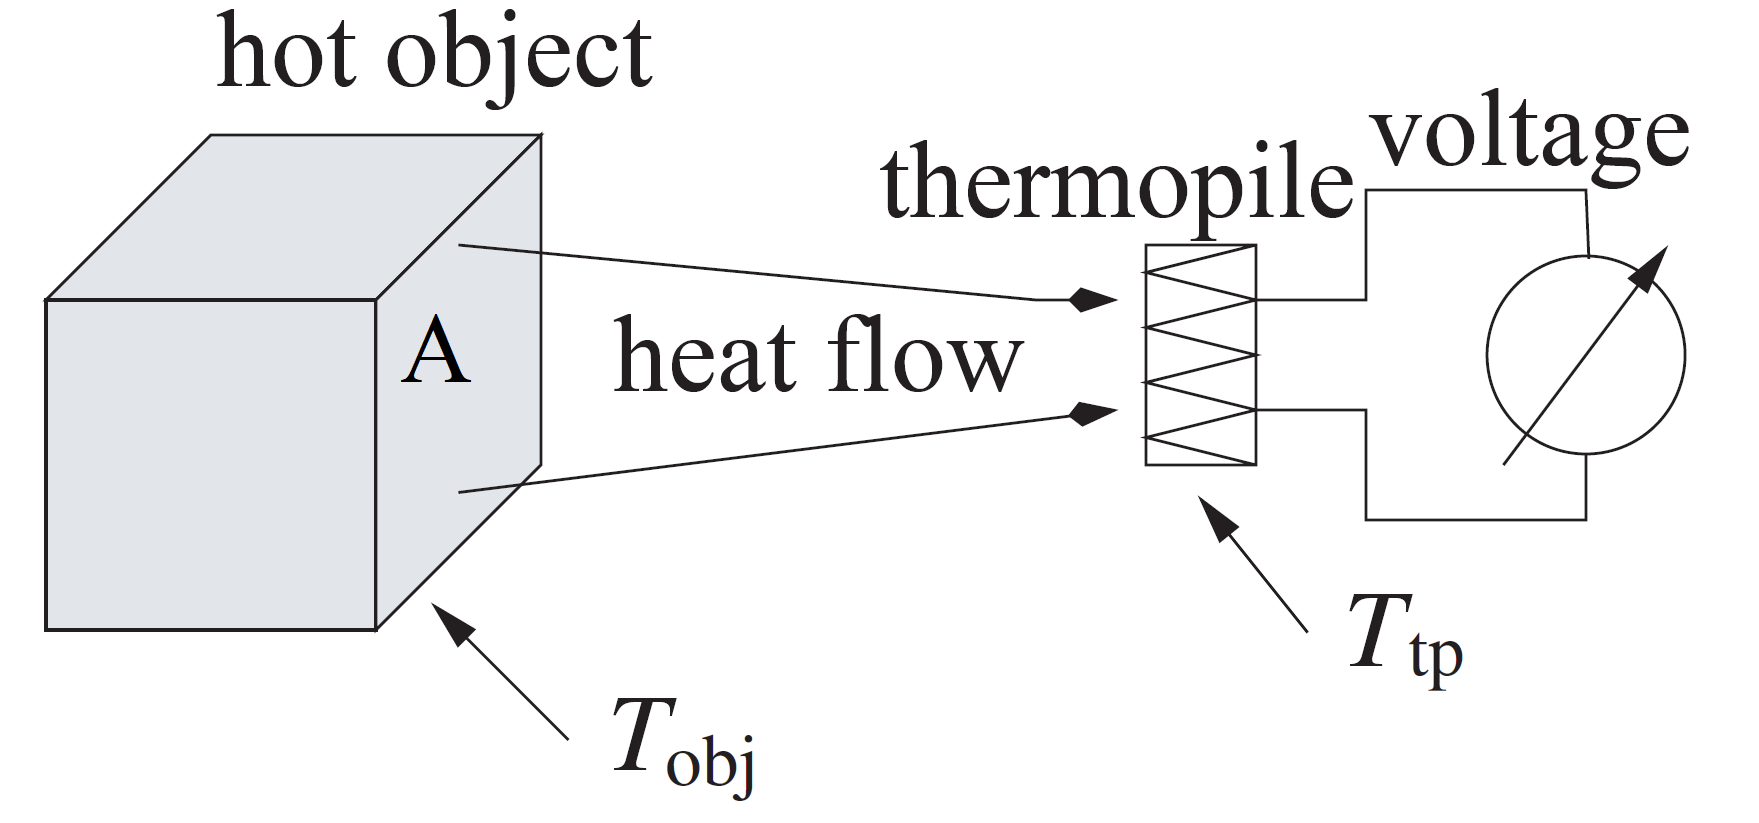
\includegraphics[width=0.5\textwidth]
	{fig/seebeck2.PNG}
	\caption[Aufbau Thermosäule]{Aufbau Thermosäule} \protect\cite{seebeck}
	\label{fig:thermosäule}
\end{figure}


Das Stefan-Boltzmann-Gesetz deutet auf eine weitere relevante physikalische Gegebenheit hin, der mit dem Emissionsgrad $\epsilon$  in Verbindung steht. Der Emissionsgrad $\epsilon$ ist ein materialabhängiger, jedoch wellenlängenunabhängier Faktor, welcher zwischen 0-1  wird. Dieser gilt für graue Körper d.h. für Körper, dessen Oberfläche auftreffende Strahlung nicht vollständig absorbieren. Diese Eigenheit gilt für alle realen Körper. Da der Emissionsgrad vom Material und dessen Oberfläche abhängt können starke Unterschiede entstehen. Im Unterkapitel \ref{subsec:Personenaufzuege} werden übliche Aufzugsmaterialien betrachtet.

Neben der Emission können auch Reflexion und Transmission von Störquellen Einfluss auf die Messwerte besitzen. In den nachfolgenden Formeln wird dies erläutert. Nach dem Energieerhaltungsgesetz \protect\cite{Thermoformeln} gilt für Transmission, Reflexion und Absorption die Formel \ref{eq4}.
\begin{equation}
\label{eq4}
\tau  + \alpha + \varphi  = 1
\end{equation}
\myequations{Schwarzer Stahler, Energieerhaltung}

Wobei bei thermischen Gleichgewicht angenommen werden kann, dass der Emissionsgrad der Absortion entpsricht.

\begin{equation}
\label{eq5}
\epsilon \approx  \alpha
\end{equation}
\myequations{Strahlung Energieerhaltung Festkörper}


Da in Aufzügen nur von Festkörper ausgegangen wird, fällt die Transmission $\tau$ aus der Gleichung. Es können lediglich Reflexionen oder die Emission eines Festkörpers Einfluss auf die einwirkende Infrarotstrahlung nehmen. Der Sensor AMG8834 ist auf einen Emissionsgrad von 0.93 kalibriert. Dies entspricht dem Emissionsgrad von Haut und Glas.\footnote[4]{ zu entnehmen Emissionsgradtabelle Anhang \ref{AnhangE}}

\section{geometrische Aspekte}
\label{sec:geometrie}

Da die Strahlungsintensität mit zunehmender Distanz im Quadrat abnimmt, spielt die Distanz zum Messobjekt eine entscheidende Rolle. Ein weiteres Punkt ist der begrenzten \ac{FOV} des Sensors von 60$^\circ$. In der nachstehenden Skizze (Abbildung \ref{fig:Geometrie}) sind die Verhältnisse perspektivisch dargestellt. Dabei wird von einer Raumhöhe von 2.10m ausgegangen.\footnote[5]{nach Standardkabine EN 81-20}  

\begin{figure}[H]
	\centering
	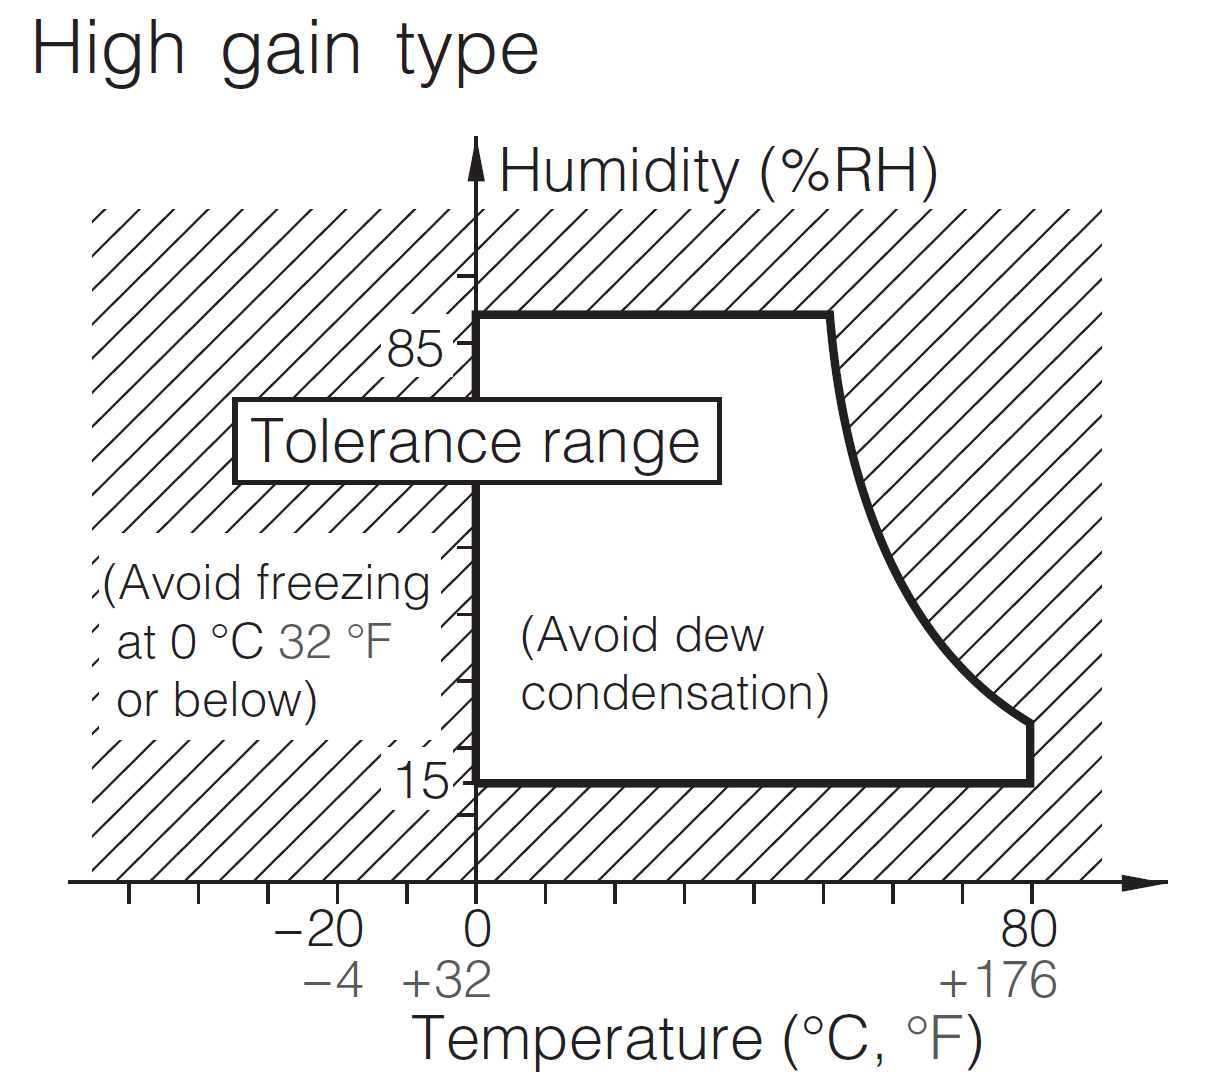
\includegraphics[width=1.0\textwidth]
	{fig/Humidity_Tolerance.PNG}
	\caption[Einfluss Luftfeuchtigkeit]{Einfluss Luftfeuchtigkeit} \protect\cite{AMG8834}
	\label{fig:Geometrie}
\end{figure}

Die räumliche Streckungen verursacht zusätzlich eine perspektivische Verzerrung, die in dieser Betrachtung nicht weiter beachtet wird. Zu sehen ist jedoch deutlich, dass bei der Messung von Personen der Messabstand zwischen 10 bis 110 Zentimeter am relevantesten ist. In diesem Bereich kann jedoch mit dem aktuellen \ac{FOV} im besten Fall eine Fläche von 0.666$m'2$ erfasst werden. Um eine Aufzugkabine mit 8 Personen\footnote[6]{Masse: (HxBxT) 2100 x 1100 x 1400 [mm]} bei mittlerem Messbereich wird im optimalen Fall ein Öffnungswinkel von 84°x 109$^\circ$ benötigt. 

Problematisch kann in diesem Zusammenhang die Abschattung des Messbereichs durch grosse Personen sein, welche zentral positioniert sind. 

 

\section{Messobjekt und Messumgebung}
\label{sec:Messobjekt}
Dieses Kapitel beschreibt die Erkenntnisse bei der Betrachtung des Messobjekts und der Messumgebung. Dabei wurden einerseits die Kennwerte von Personen zusammengetragen, sowie die Messumgebung auf Störquellen und Einflussfaktoren begutachtet. Dank der Firma ARLEWO AG konnten unterschiedliche Aufzüge vermessen und bewertet werden. 

\subsection{Personen}
\label{subsec:Personen}

Die Reaktionen im menschlichen Körper sind auf eine Kerntemperatur von 37 °C. Am kältesten ist die Haut, die etwa 4 bis 7 Kelvin (Grad) kälter ist. Die Aufteilung der verschiedenen Arten der Wärmeabgabe beträgt bei einem ruhenden Menschen in einer Umgebung von 20 °C:


\begin{itemize}
	\item 46 \% Strahlung
	\item 33 \% Konvektion\footnote[7]{Konvektion bezeichnet die Wärmeabgabe an
		das umgebende Medium, in der Regel Luft}
	\item 19 \% Schwitzen
	\item \space  2 \% Atmung
\end{itemize}

Die Höhe der Wärmeabgabe hängt im wesentlichen von der Schwere der Tätigkeit und von der Größe der Körperfläche ab. Daraus folgt, dass größere Personen mehr Wärme abgeben. Strahlung und Konvektion nehmen mit zunehmender Umgebungstemperatur bis zum Wert null bei 36$^\circ$ C ab. Hat die Umgebung die Körpertemperatur erreicht, kann folglich durch Strahlung und Konvektion keine Wärme mehr abgeführt werden. In einer Umgebung mit Temperaturen oberhalb 37$^\circ$ C kann also die Wärme nur noch durch Schwitzen abgeführt werden.\protect\cite{MenschWaerme}

Da die Personenerkennung auf Temperaturdifferenzen beruht, kann bei einer Umgebungstemperatur um 37$^\circ$C eine Personen nicht mehr zweifelsfrei von der Umgebung differenziert werden.
\newpage
Ein weiterer Aspekt, der sehr stark ins Gewicht fällt, ist die Art der Bekleidung. In Abbildung \ref{fig:Waermebild} und Abbildung \ref{fig:Waermebild2} ist deutlich zu sehen, dass das thermische Profil einer Person durch die Bekleidung stark variiert.
\begin{figure}[!ht]
	\centering
	\begin{minipage}[b]{0.4\linewidth}
		\centering	
		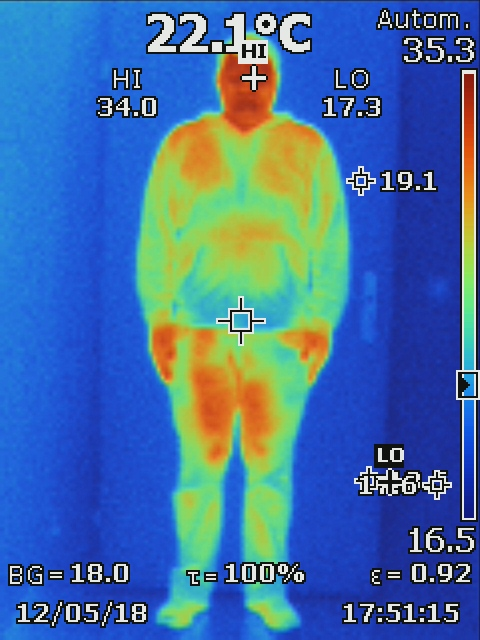
\includegraphics[width=0.8\linewidth]{fig/waermebild1.jpg}
		\captionof{figure}[Wäermebild eines \\Probanden]{Wärmebild eines Probanden}
		\label{fig:Waermebild}
	\end{minipage}
	\hfill
	\begin{minipage}[b]{0.4\linewidth}
		\centering
		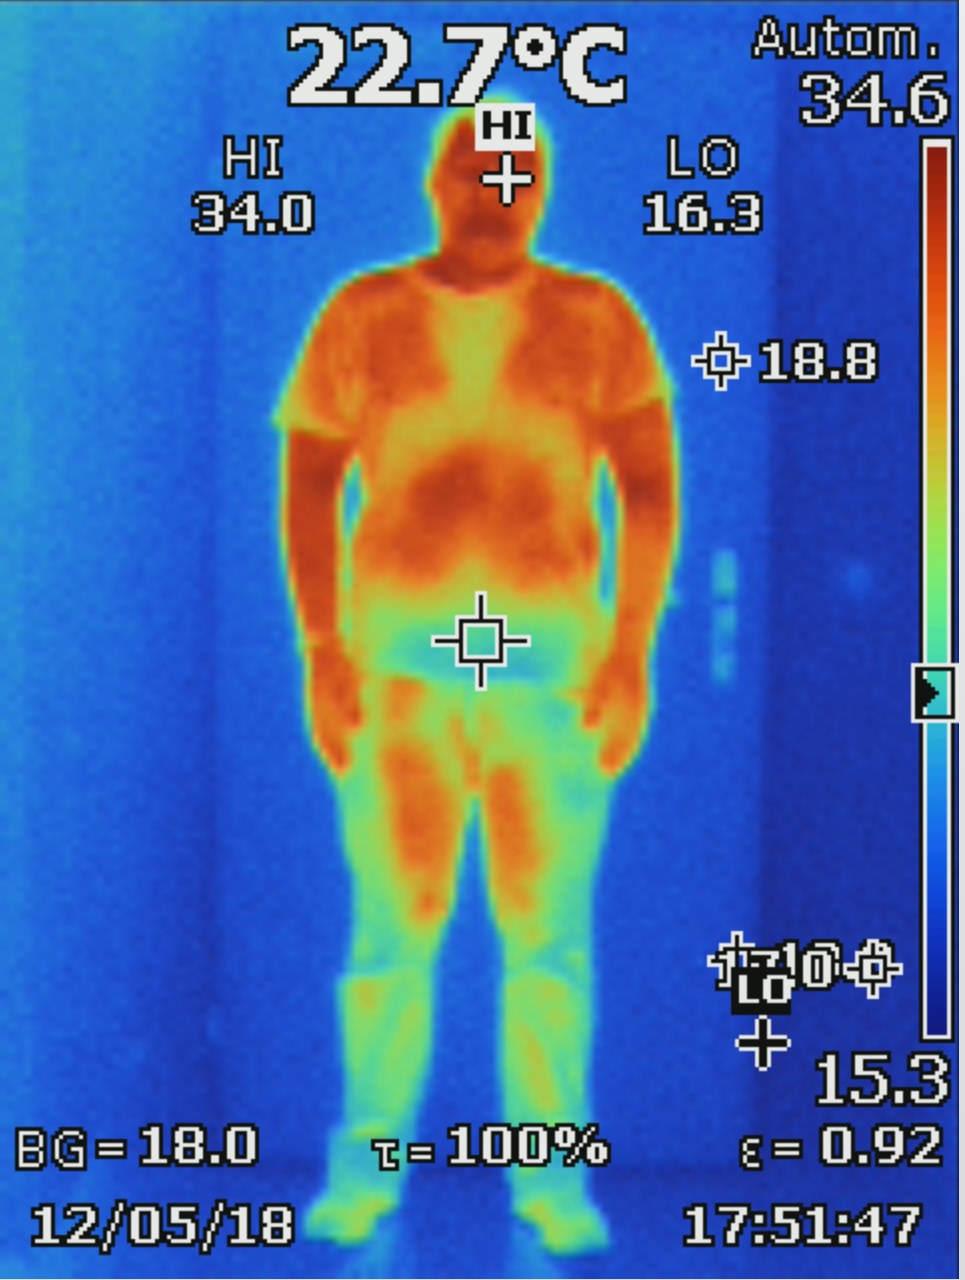
\includegraphics[width=0.8\linewidth]{fig/waermebild2.png}
		\captionof{figure}[Wäermebild eines\\Probanden]{Wärmebild eines Probanden}
		\label{fig:Waermebild2}	
	\end{minipage}
\end{figure}

 Unbekleidete Zonen sind üblicherweise die wärmsten Regionen. Die Bekleidung hängt von der Art ab und variert zwischen Hauttemperatur und Umgebungstemperatur. Im Falle von einem Umgebungstemperaturwechsel besitzt die Kleidung eine verzögerte Reaktion bis sich die neue Temperatur einstellt. Dies ist insofern relevant, weil bei einem Wechsel vom Aussenbereich zu einem beispielsweise klimatisierten Innenbereich, die Bekleidung im Verhältnis zur Umgebungstemperatur abweicht.

\subsection{Personenaufzüge}
\label{subsec:Personenaufzuege}
In diesem Unterkapitel wurde der Personenaufzug als Messobjekt näher betrachtet. Neben räumlichen Parametern wie Höhe, Grundfläche und Volumen spielen vor allem die Oberflächenbeschaffenheit bzw. das Oberflächenmaterial Rolle. Weitere Einflussfaktoren finden sich in der Umgebungstemperatur und der verbauten Leuchtmittel.

Wie bereits in Unterkapitel \ref{subsec:Strahlungstheorie} erläutert, besitzten die Materialien in einem Personenaufzug zum Teil stark abweichende Emisisonsgrade. Dies verursacht, dass die gemesssen Temperaturen nicht den effektiven Temperaturen entsprechen. 

In Abbildung \ref{fig:Edelstahlgewalzt} und \ref{fig:Edelstahlmatt} sind 
\begin{figure}[H]
	\centering
	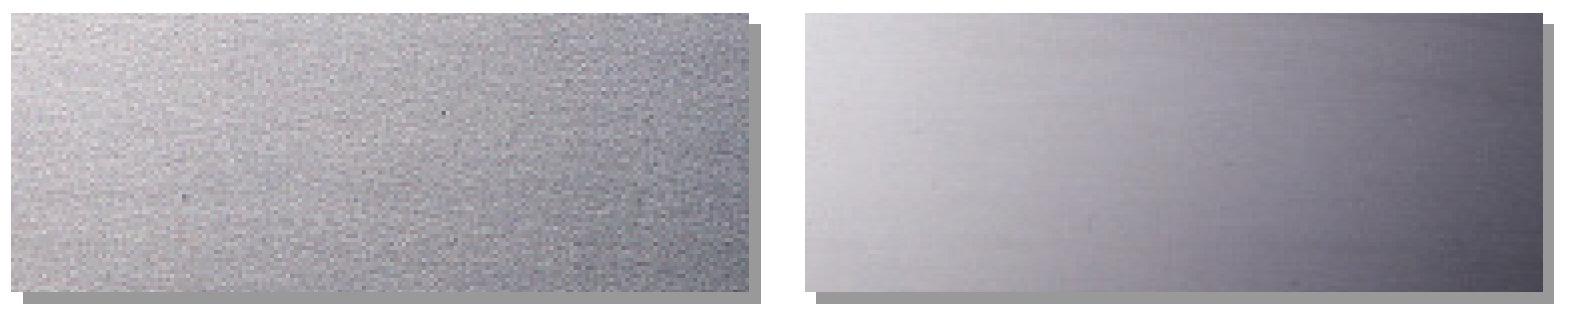
\includegraphics[width=0.8\textwidth]
	{fig/Edelstahl_gewalzt.PNG}
	\caption[Edelstahl warmgewalzt]{Edelstahl warmgewalzt} \protect\cite{Edelstahl}
	\label{fig:Edelstahlgewalzt}
\end{figure}
\begin{figure}[H]
	\centering
	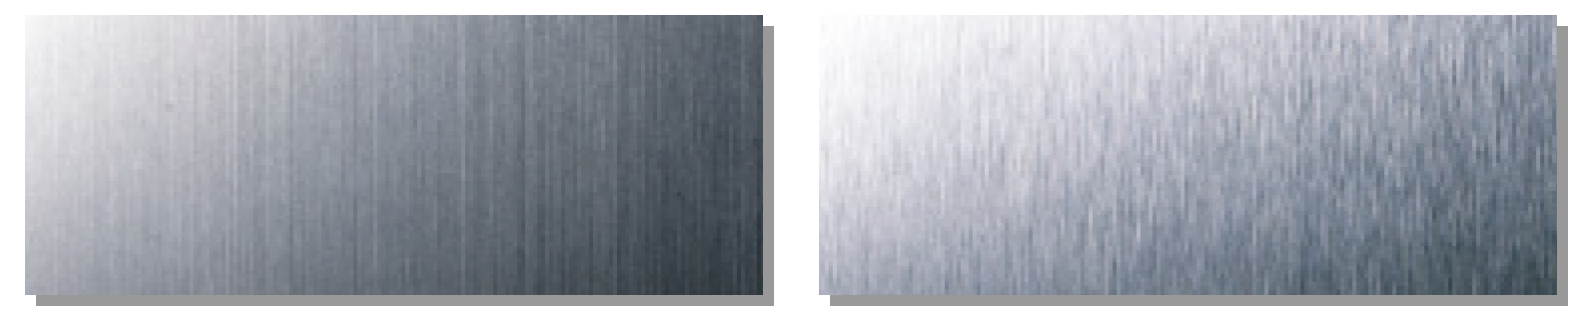
\includegraphics[width=0.8\textwidth]
	{fig/Edelstahl_matt.PNG}
	\caption[Edelstahl kaltgewalzt]{Edelstahl kaltgewalzt} \protect\cite{Edelstahl}
	\label{fig:Edelstahlmatt}	
\end{figure}




\begin{figure}[H]
	\centering
	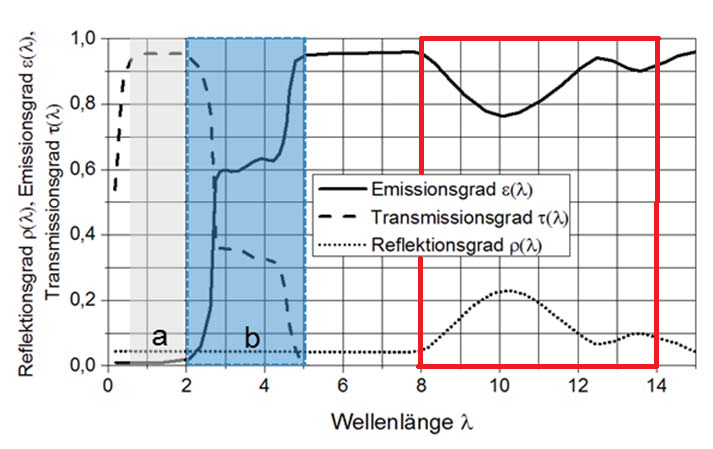
\includegraphics[width=0.8\textwidth]
	{fig/Glas_bearbeitet.png}
	\caption[Emissionsgrad in Abhängikeit zur Wellenlnge]{Emissionsgrad in Abhängikeit zur Wellenlänge von Glas} 
	\label{fig:Glas}	
\end{figure}

\section{Fazit}

Die Personenerkennung in Aufzügen mit \ac{PIR} Sensoren ist am meisten von der Individualität einer Person abhängig. Faktoren wie Körpertemperatur, Körpergröße und Bekleidung verursachen enorme Differenzen. Dadurch kann kein einheitliches Profil erstellt werden. Da Personenaufzüge Normgrössen besitzen, besteht mit dem AMG8834 durch den begrenzten \ac{FOV} nur einen begrenzten Messbereich. Entsprechende Linsenanpassung können die PRoblematik lösen. 
Weitere physikalische Gegebenheiten wie die Umgebungstemperatur oder indirekte Sonneneinstrahlung bewirken veränderte Bedingungen für den Messbereich, welche bei einer Messeinheit berücksichtigt werden müssen. Die verwendeten Leuchtmittel besitzten, soweit Einfluss, da deren Betriebstemperatur      


